\documentclass{article}
\setlength{\oddsidemargin}{0 in}
\setlength{\evensidemargin}{-0.25 in}
\setlength{\topmargin}{-0.6 in}
\setlength{\textwidth}{6.5 in}
\setlength{\textheight}{8.5 in}
\setlength{\headsep}{0.75 in}
\setlength{\parindent}{0 in}
\setlength{\parskip}{0.1 in}

% ===== PACKAGES =====
\usepackage{amsmath,amssymb}
\usepackage{color}
\usepackage{subfigure}
\usepackage{mdframed}
\usepackage{changepage}
\newmdenv[
  topline=false,
  bottomline=false,
  skipabove=\topsep,
  skipbelow=\topsep
]{siderules}
\renewcommand{\abstractname}{}

% ===== VARIABLES =====
\def \R{\mathbb{R}}
\def \Pr{\mathbb{P}}
\def \D{{\rm D}}
\def \N{{\rm N}}
\def \xx{{\boldsymbol{\rm x}}}
\def \y{{\rm y}}

% ===== HEADER BOX =====
\newcommand{\lecture}[2]{
\pagestyle{myheadings}
\thispagestyle{plain}
\newpage
\noindent
\begin{center}
\rule{\textwidth}{1.6pt}\vspace*{-\baselineskip}\vspace*{2pt} % Thick horizontal line
\rule{\textwidth}{0.4pt}\\[1\baselineskip] % Thin horizontal line
\vbox{\vspace{2mm}
\hbox to 6.28in { {\bf CS 760: Machine Learning} \hfill Spring 2024 }
\vspace{4mm}
\hbox to 6.28in { {\Large \hfill #1  \hfill} }
\vspace{4mm}
\hbox to 6.28in { {\scshape Authors:}  #2 \hfill }}
\vspace{-2mm}
\rule{\textwidth}{0.4pt}\vspace*{-\baselineskip}\vspace{3.2pt} % Thin horizontal line
\rule{\textwidth}{1.6pt}\\[\baselineskip] % Thick horizontal line
\end{center}
\vspace*{4mm}
}

% ===== Jed's Defined Stuff ======
\DeclareMathOperator*{\argmin}{arg\!\min}
\DeclareMathOperator*{\argmax}{arg\!\max}
\usepackage{siunitx}
\usepackage{enumitem} % used to make alphabetical lists instead of numbered ones
\usepackage{mathtools}
\usepackage{graphicx}
\usepackage{caption}
\usepackage{hyperref}

% =============== DOCUMENT ===============
\begin{document}
\lecture{Convolutional Neural Networks}{Jed Pulley \& Keshav Sharan Pachipala}

\begin{center}
{\Large {\sf \underline{\textbf{DO NOT POLLUTE!}} AVOID PRINTING, OR PRINT 2-SIDED MULTIPAGE.}}
\end{center}

% \begin{abstract}
% Write your abstract here
% \end{abstract}

\section{Introduction}
    In recent years, Convolutional Neural Networks (CNNs) have emerged as a cornerstone technology in the field of deep learning, particularly in the domain of computer vision. CNNs are adept at extracting intricate patterns and features from spatially structured data. Some fields that benefit from CNNs include image classification, object detection, and medical image analysis.
    
    In this paper, we won't go into the exact specifics of what a convolution is since it's slightly different in the discrete and continuous cases, as well as slightly different in a CNN context, but if you're really curious about it, 3Blue1Brown has some excellent videos visually explaining the mathematical concepts behind a convolution in his videos linked below [1] and [2].

\section{Understanding the Architecture}
    \subsection{NNs vs CNNs}
        Neural Networks and CNNs are similar in many ways, but also have drastically different architectures. From a high level, the classic neural network example has an input layer, hidden layers, and an output layer, shown below:
        
        \begin{center}
            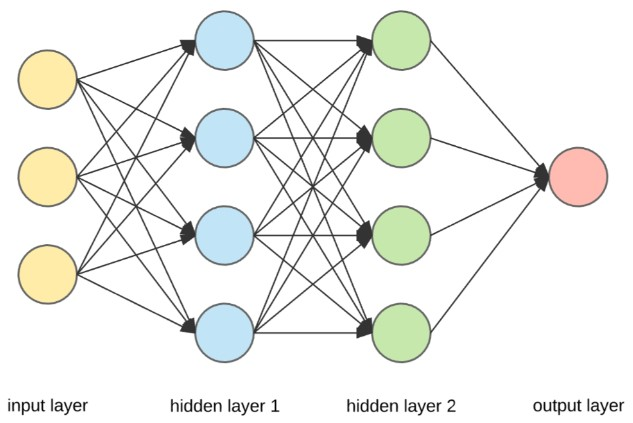
\includegraphics[scale=0.5]{images/NN.jpg}    
        \end{center}
        
        However, the architecture of a convolution neural network looks much different. There isn't one right way to structure it, but typically a CNN will have the input, a few convolution and pooling layers, a flattening step, and then finally a fully connected layer that leads to an output, as shown below. Notably, how you structure your CNN is an area of active research today.
        
        \begin{center}
            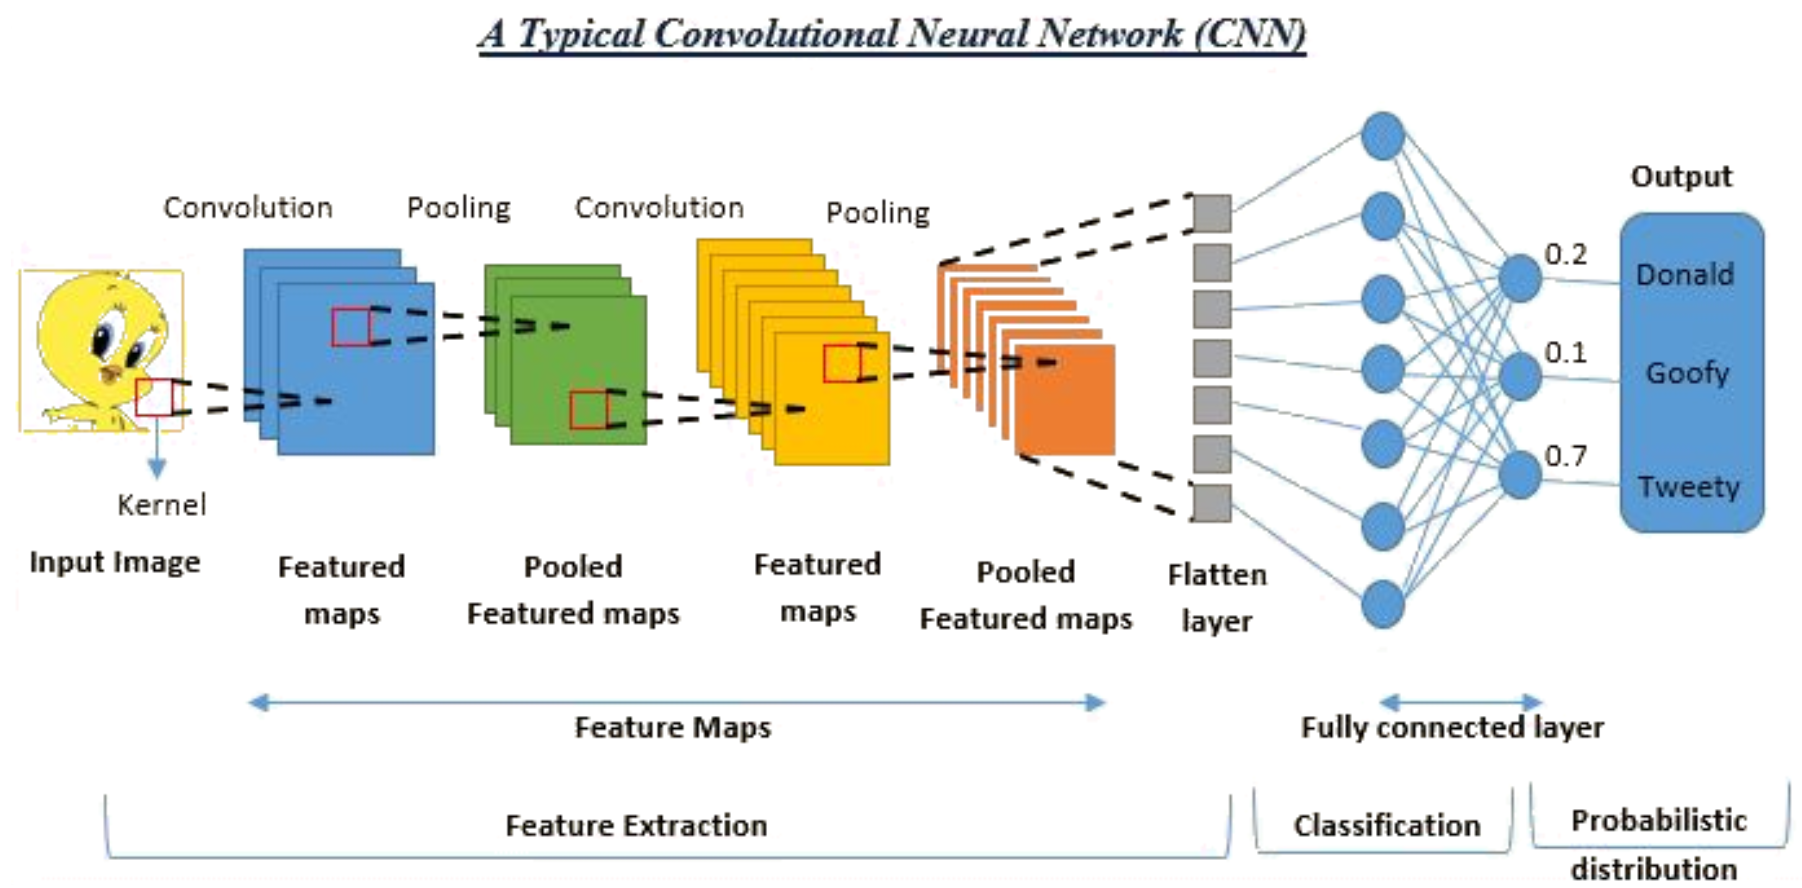
\includegraphics[scale=0.3]{images/CNN.jpg}
        \end{center}
        
        Another important distinction between the two is that for a CNN, the weights that we are trying to learn are the kernels themselves, along with a bias term.

    \subsection{Kernels}
        Fundamental to the idea of convolutions are kernels. In the context of CNNs, the words kernel and filter are interchangeable, but for this paper we'll stick with kernel. In the 2D image processing case, a kernel takes the form of a square grid of odd dimensions. So for example 3x3, 5x5, or 9x9. These days, you'll almost exclusively see kernels of dimensions 3x3 or even 1x1. Kernels are odd so that they have a center, but they don't necessarily have to be. The reason for 3x3 goes back to 2012 when the ImageNet competition was in full swing. Briefly put, ImageNet was a challenge to see who could most efficiently and accurately classify a dataset of more than 14 million hand-annotated images into roughly 20,000 categories. In 2012, a model called AlexNet swept the competition outperforming all others by significant margins. AlexNet pioneered CNNs for the image processing task. One of the reason's for it's success was it's heavy use of 3x3 kernels. However, it wasn't until the next year when an optimized version of AlexNet, called ZFNet, took it a step further and used 3x3 kernels in almost every layer. There are many different ways to determine your kernel size, but starting out with 3x3 is a safe bet.
        
    \subsection{Convolution Layer}
        The convolution layer is the defining aspect of a CNN. To actually perform the convolution step means sliding the kernel across the image pixel by pixel, multiplying each element with it's overlapping counterpart and summing them up to produce the output. The output is a single pixel in the output image/matrix. You scroll through the entire image performing the same operation until complete. Since the kernel extends past the boundaries when it's near the edges, often times padding is added. This step is shown in the image below:
        
        \begin{center}
            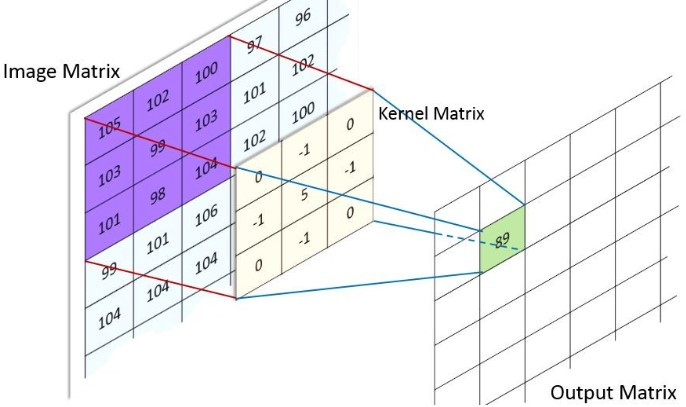
\includegraphics[scale=0.6]{images/kernel.jpg}
        \end{center}
        
        Since the operative pixel is the center of the kernel, convolution runs into the issue of overlapping the image. So to avoid this, with a 3x3 kernel for example, a single pixel of padding is added to the image so that the kernel will fit in the first row/column.

        The general expression for a convolution is as follows:
        \[ g(x, y) = \omega \ast f(x, y) = \sum_{i=-a}^{a} \sum_{j=-b}^{b} w(i, j) * f(x - i, y - j) \]
        where $g(x, y)$ is the filtered image, $f(x, y)$ is the original image, and $\omega$ is the kernel.

        One of the biggest advantages of a convolution is that when applied to structured data, it can take advantage of the spatial relationship between said data. Whereas normally that relationship would be lost when flattened out and pumped through a regular neural net.

    \subsection{Pooling Layer}
        The next step of the CNN is to perform pooling on the input image. There are many methods used for this, but the most common are max pooling and average pooling. For pooling, you again take a kernel (this one doesn't need to have odd dimensions) and scan it across the image. However this time, instead of going pixel by pixel, you stride over the image. And for each step, in the max pooling case, you take the maximum value in the overlapping kernel region:
        
        \begin{center}
            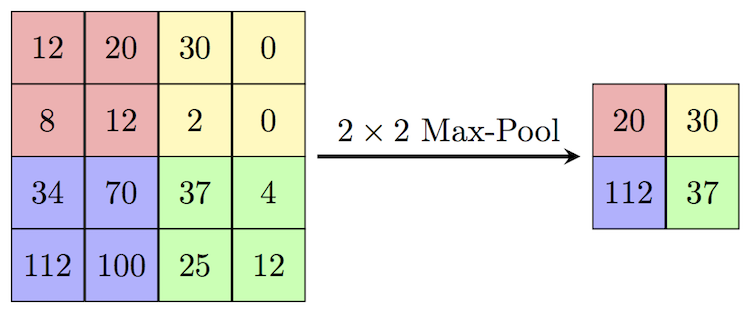
\includegraphics{images/maxpool.png}
        \end{center}
        
        In the case of average pooling, the process is exactly the same excpet instead of taking the maximum, you average the values out and use that. Often times, you'll see a kernel size of 2x2 and a "stride" of 2 for pooling. This means that you'll examine a 2x2 area, choose the maximum (or average) of that area, and then return it. After that, you stride the kernel over two steps and repeat over the entire image. This has two main functions: down sampling and shift-invariance
        
        \begin{enumerate}
            \item \textbf{Down Sampling}: This step reduces the overall size of your data while also preserving the main features from the previous layers. So moving forward, you are left with a smaller, more informationally dense input that gets propagated into further layers. This leads to more computational efficiency.
            \item \textbf{Shift-Invariance}: This effect is slightly less stated, but still important. If, for example, the kernel's job was to detect whiskers on a cat, down-sampling makes the convolution step slightly more invariant to shifts in the image. Since pooling carries forward important features and reduces the area, you get the same feature but are less concerned with where in the image that feature was found. This effect is marginal, but still leads to more robust classification.
        \end{enumerate}

    \subsection{Flattening \& Fully Connected Layer}
        The flattening step appears after the convolutional and pooling layers. It acts as a bridge between the convolutional/pooling layers, which extract spatial features, and the fully connected layers, which perform classification or regression tasks. After flattening, a fully connected layer is hooked up to the output layer with it's own weights and biases.
        
    \subsection{Output Layer}
        The output layer is the same as what you would find in a regular neural network. For a classification task, the outputs would be the confidence of that specific class. However, this layer is generalizable to the specific needs of whatever flavor of CNN you are implementing.

    \subsection{Activation Functions}
        Like any neural network, CNNs use activation functions to introduce non-linearity into the system. Common activation functions include Tanh, ReLU, and the Sigmoid functions, as shown below:

        \textbf{Sigmoid}
        \[ \sigma(z) = \frac{1} {1 + e^{-z}} \]

        \textbf{ReLU}
        \[ Relu(z) = max(0, z) \]

        \textbf{Tanh}
        \[ tanh(x) = \frac{e^x - e^{-x}}{e^x + e^{-x}} = \frac{1 - e^{-2x}}{1 + e^{-2x}} \]

    \subsection{Batch Normalization}
        To quote from Younesi et al. [4]:

        \begin{quote}
            Batch Normalization is a technique that helps stabilize and accelerate the training of CNNs. It normalizes the activations of each layer by centering and scaling the values using the mean and variance of each mini-batch during training. This process reduces internal covariate shifts, making the optimization process smoother and enabling the use of higher learning rates. By normalizing activations, Batch Normalization allows for more aggressive learning rates, which leads to faster convergence and improved model generalization. Additionally, it acts as a regularizer, reducing the need for other regularization techniques like dropout. Overall, Batch Normalization has become a standard component in CNN architectures, contributing to faster training, improved model performance, and increased ease of hyperparameter tuning. Its widespread adoption has significantly contributed to the success of modern CNNs in various CV and NLP applications.
        \end{quote}

    \subsection{Backpropagation}
        Unlike traditional neural networks, both the forward pass and the backprop pass of a convolutional layer are convolutions [5].

        I don't want to go into further detail as my explanation would pale in comparison to Pavithra Solai's explanation in the article linked at [5] below. If you're interested in an excellent visual and intuitive understanding of CNN backprop, I highly recommend it.
        
\section{Advanced CNN Architectures}
    \subsection{VGGNet}
        In traditional neural networks, increasing the number of layers to deepen the network allows for learning more complex features, which is crucial for advanced image recognition tasks. VGG, which was developed by the Visual Graphics Group, pushed this concept to new heights by significantly increasing network depth using an architecture with up to 19 layers. This  helped establish new benchmarks in accuracy. However, such deep networks also introduced some obvious challenges, including increased computational demands and a higher propensity for overfitting, requiring innovations in training and regularization techniques.
        
        VGG16's architecture is characterized by its uniformity. It exclusively uses 3x3 convolutions with a stride of 1 and max pooling of 2x2 with a stride of 2. Such simplicity for ease of understanding and implementation, and its depth, enables the learning of a rich hierarchy of features. It has been used as a baseline for many computer vision tasks and is still used as a feature extractor for many other types of problems beyond classification.

        The convolutional layers, depicted as blue blocks in our diagram, apply filters to its input. The number of filters grow as we progress deeper into the network, from 64 in the first layers to 512 in the deeper layers. The notation 224x224x64, for example, represents the spatial dimensions of the feature map followed by the depth, indicating the number of filters.

        After each convolution, we apply the ReLU activation function to introduce non-linearity, allowing the network to learn complex patterns.

        Next, the max pooling layers, shown in red, reduce the spatial dimensions by half—importantly decreasing the feature map size to manage computational resources while retaining critical features. Each pool operates over a 2x2 pixel window with a stride of 2.

        As we approach the network's end, the spatial feature maps are flattened, leading to fully connected layers. Finally, the output layer, which connects the last fully connected layer to a 1000-unit layer, corresponds to the number of classes in ImageNet. Here, we use a softmax function to calculate a probability distribution over class labels, defined mathematically as \( P(y = i \mid \mathbf{x}) = \frac{e^{x_i}}{\sum_{j} e^{x_j}} \), where \( x_i \) is the input to a neuron corresponding to class i.
        
        \begin{center}
            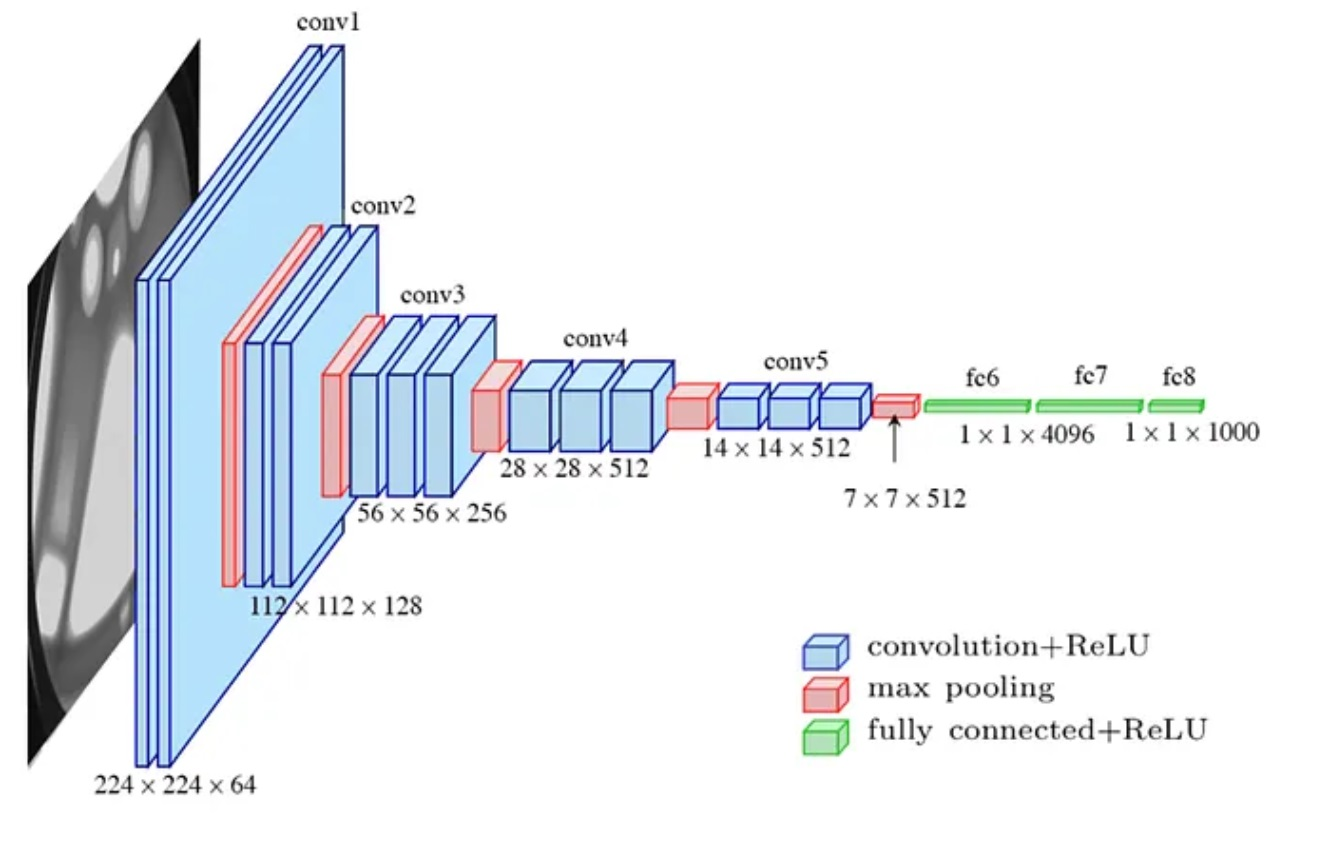
\includegraphics[scale=0.4]{images/VGG.jpg}
        \end{center}
        
    \subsection{GoogleNet (InceptionNet)}
        
        While deepening the architecture of neural networks theoretically enhances their ability to learn more complex features, it also complicates the training process and increases the computational load. GoogleNet, or InceptionNet, addresses these challenges by introducing a novel architecture known as the 'inception module'. This module allows the network to look at the same input through multiple scales simultaneously, and significantly reduces the parameter count while maintaining, if not increasing, the depth and width of the network. This approach not only preserves the capacity to learn complex features but does so with enhanced efficiency, mitigating the issues of computational expense and overfitting seen in simpler deep networks.
        
        \begin{center}
            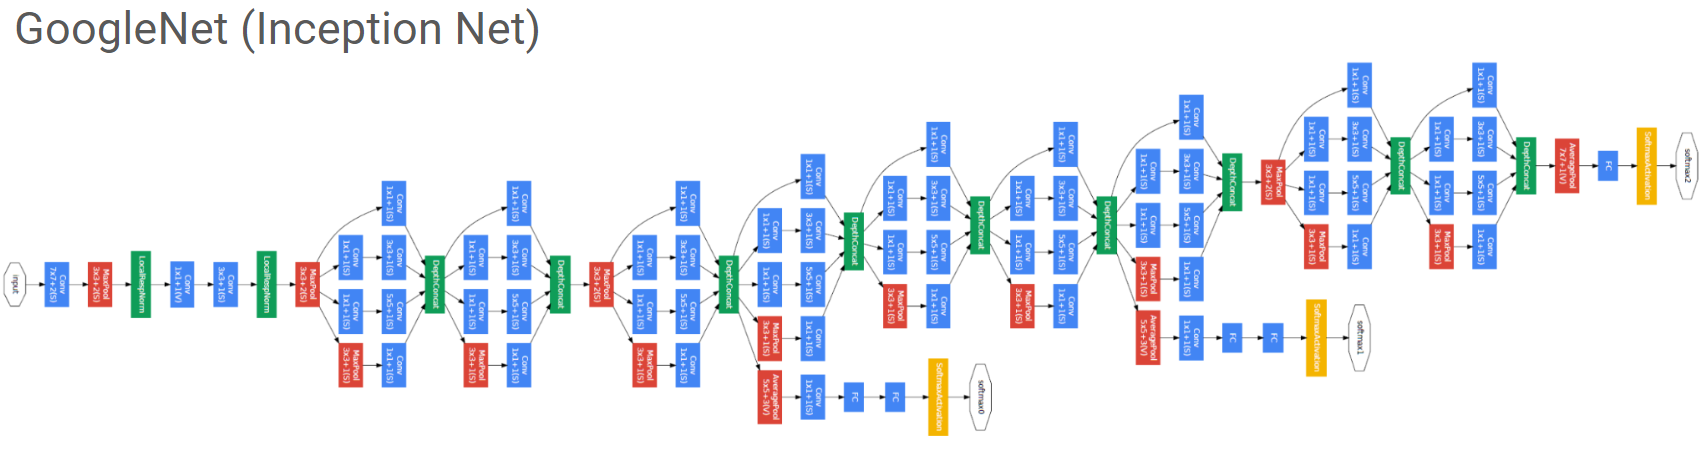
\includegraphics[scale=0.35]{images/GoogleNet.png}
        \end{center}
        
        This increased efficiency facilitated by the inception modules is achieved by performing multiple convolutions of different sizes simultaneously, creating a kind of "network within a network", greatly reducing the number of parameters compared to VGG. Finally it employs auxiliary classifiers during training to inject gradients at lower layers to combat vanishing gradients.

        \begin{center}
            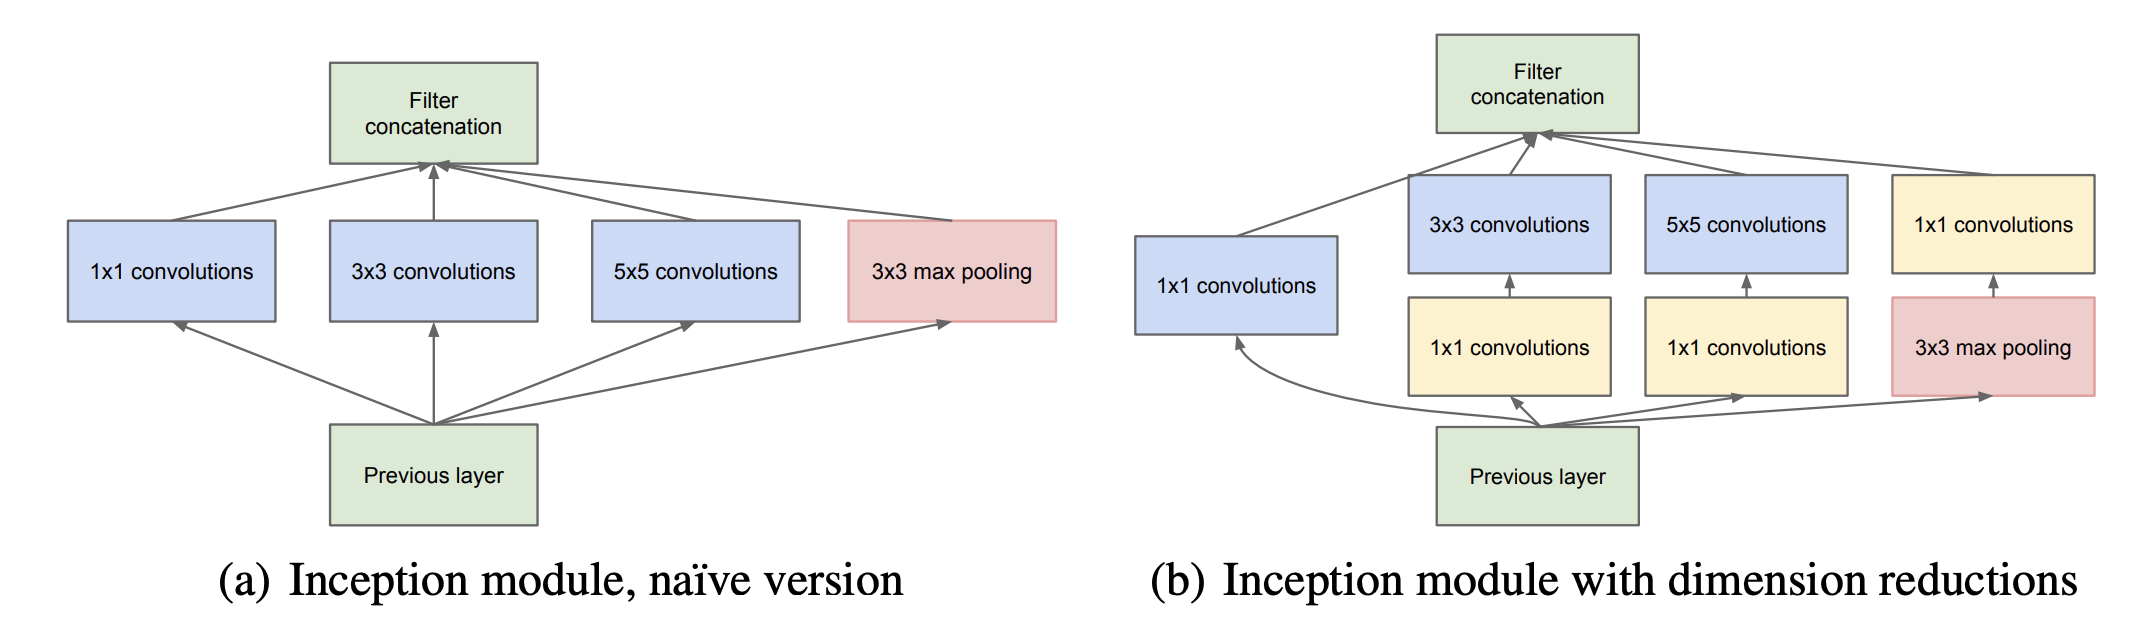
\includegraphics[scale=0.2]{images/inceptionmodule.png}
        \end{center}
        
        The Inception module consists of multiple filter operations happening simultaneously. It combines 1x1, 3x3, and 5x5 convolutional filters along with 3x3 max pooling. This multi-scale processing allows the network to capture details at various extents from the same input level.

        Crucially, 1x1 convolutions used within the module are for dimension reduction before larger convolutions. This reduces the computational cost without losing critical information, serving both as bottleneck layers that compress the input features and as network regularization to prevent overfitting.

        After processing through different paths, all outputs are concatenated along the depth dimension. This concatenated volume feeds into the next layer, providing a rich, combined feature set that integrates diverse patterns and scales detected within the input.
        
        Meanwhile, auxiliary classifiers are additional classifiers added to intermediate layers of the network. Their role is to provide an additional training signal from these intermediate layers directly, rather than relying solely on the gradient signal propagated from the final output layer.
 
    \subsection{ResNet (Residual Network)}
        Here we have ResNet which uses "residual connections" to allow gradients to bypass layers, which helps in training very deep networks by alleviating the vanishing gradient problem. The skip connections perform identity mapping, and their outputs are added to the outputs of the stacked layers. They can support deeper architectures as they can be built with a much greater depth than previous models while still maintaining trainability.  (e.g., ResNet-50, ResNet-101, ResNet-152) Finally, they offer reduced complexity. Despite being deeper, they tend to have fewer parameters and are less complex than VGG due to the lack of fully connected layers.

        \begin{center}
            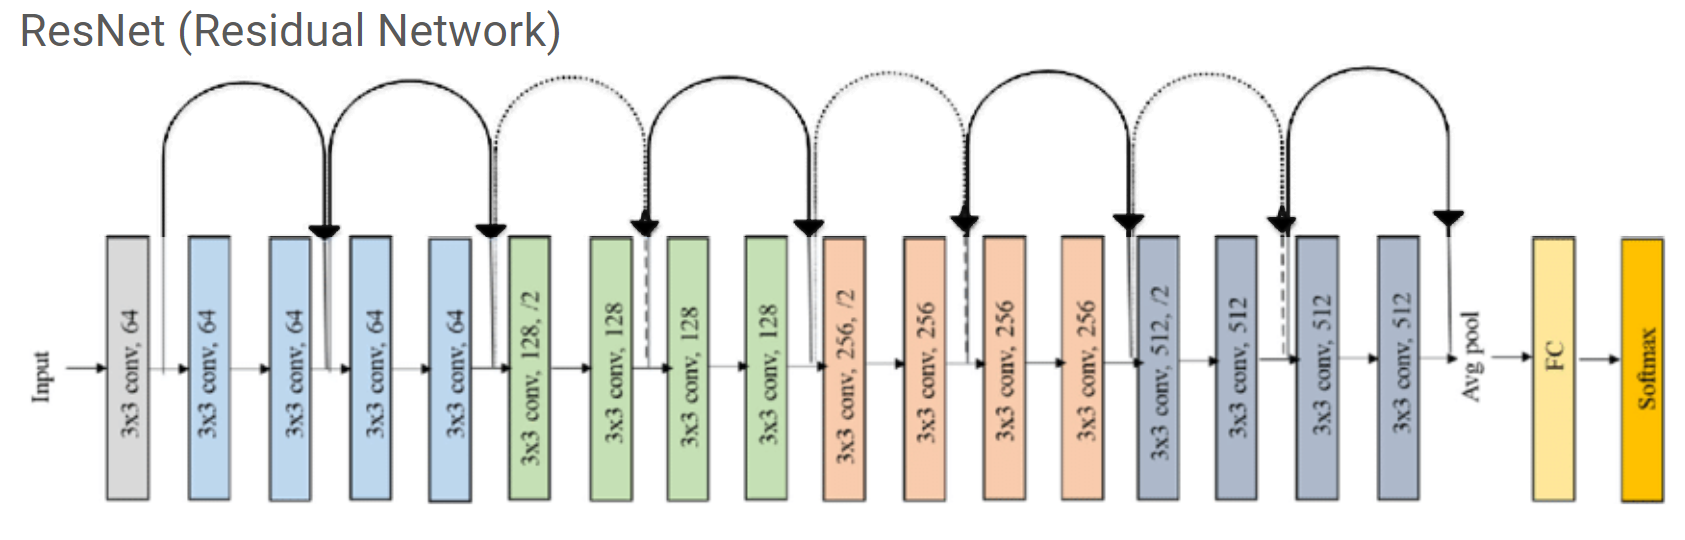
\includegraphics[scale=0.35]{images/ResNet.png}
        \end{center}

        The above image of ResNet 18 depicts these components in a sequence that corresponds to how data flows through the network: starting from the input, passing through various convolutional and pooling layers, and eventually leading to the output where a prediction is made. The "shortcut" connections are what make this network "residual"; they skip one or more layers and help preserve the gradient signal throughout the network.

        \begin{center}
            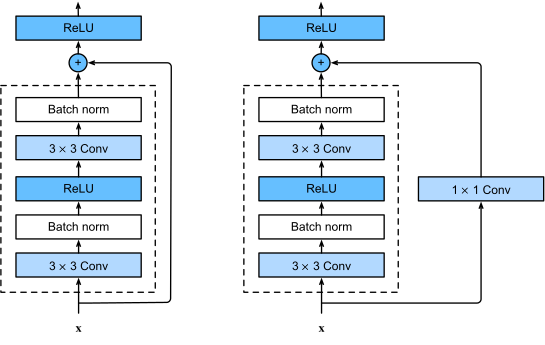
\includegraphics[scale=0.35]{images/resnet-block.png}
        \end{center}

        Convolutional layers are the core building blocks of ResNet. These layers are represented as rectangular blocks, each labeled with the filter size, such as '3x3', and the number of filters, like 64 or 128. They are the primary building blocks of ResNet, applying various filters to extract features like edges, textures, and shapes.

        As mentioned above, the defining features of this architecture are the curved arrows that bypass one or more layers. They directly connect the input of a layer block to its output, facilitating deeper networks by allowing gradients to flow freely through the architecture.

        All convolutions are followed by batch normalisation which are then followed by ReLu activation functions. The final average pooling and fully connected layer lead to the softmax that outputs a probability distribution over the classes.
        
\section{Trends \& Future Directions}
    \subsection{Accuracy}
    
        \begin{center}
                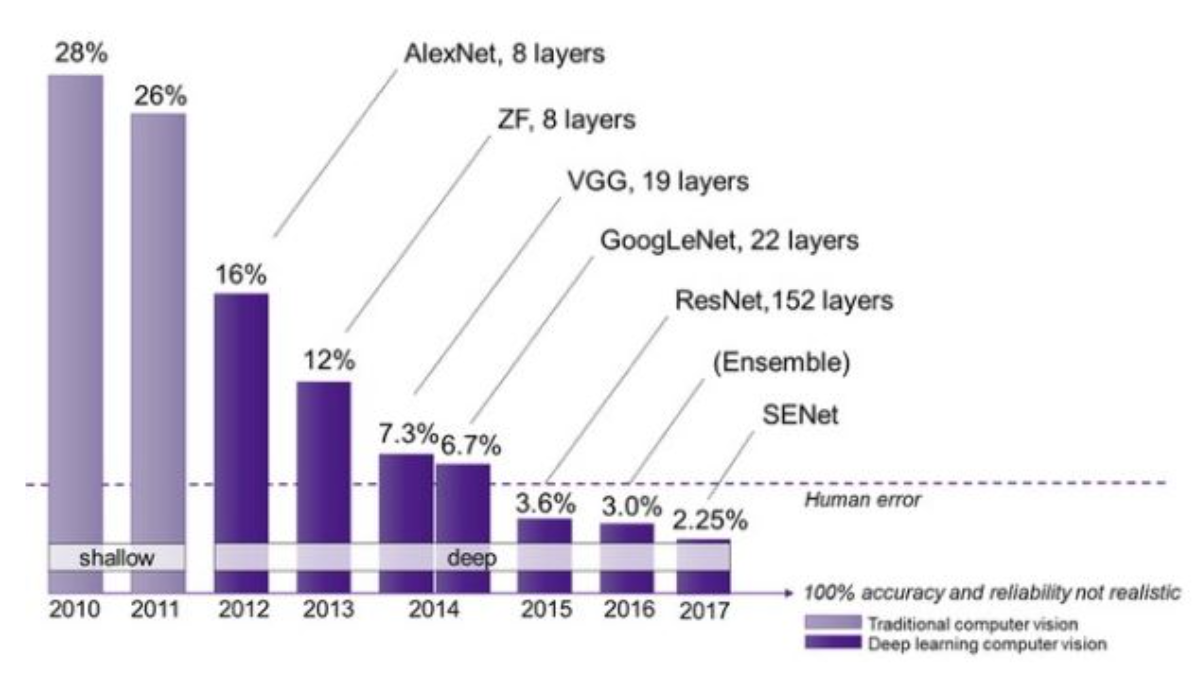
\includegraphics[scale=0.3]{images/accuracy.png}
        \end{center}
        
        VGG showed that depth matters for feature hierarchy. InceptionNet introduced computational efficiency with parallel convolutions and ResNet enabled the training of even deeper networks through skip connections for better classification performance. As we can see, CNNs have become increasingly accurate over the years and are currently more accurate than humans, who are estimated to have around 5\% error rate. Since 100\% accuracy is not realistic, what else can be improved?        

    \subsection{Potential Improvements}
        \begin{itemize}
            \item \textbf{Efficiency and Optimization}: Streamline CNNs to require fewer computational resources to enable deployment on low-power, edge computing devices.
            \item \textbf{Robustness and Generalization}: Increase CNN resilience to adversarial attacks and their ability to perform well on unseen and noisy data.
            \item \textbf{Transfer Learning and Few-Shot Learning}: Adapt CNNs to new tasks with minimal data through methods like transfer and few-shot learning.
            \item \textbf{Interpretability and Explainability}: Currently CNNs operate like back boxes. We have to make CNN decisions transparent and understandable to ensure trustworthiness and compliance in critical applications in industries like the automotive and the medical industry.
        \end{itemize}
    
\section{Resources}
    \textbf{[1]} 3Blue1Brown - But What is a Convolution? \\
    \url{https://www.youtube.com/watch?v=KuXjwB4LzSA&t=1s}
    
    \textbf{[2]} 3Blue1Brown - Convolutions | Why X+Y in probability is a beautiful mess \\
    \url{https://www.youtube.com/watch?v=IaSGqQa5O-M}
    
    \textbf{[3]} far1din - Convolutional Neural Networks from Scratch | In Depth \\
    \url{https://www.youtube.com/watch?v=jDe5BAsT2-Y}
    
    \textbf{[4]} Younesi, A., Ansari, M., Fazli, M. A., Ejlali, A., Shafique, M., \& Henkel, J. (2024). A Comprehensive Survey of Convolutions in Deep Learning: Applications, Challenges, and Future Trends. arXiv preprint arXiv:2402.15490 \\
    \url{https://arxiv.org/abs/2402.15490}

    \textbf{[5]} Pavithra Solai - Convolutions and Backpropagations \\
    \url{https://pavisj.medium.com/convolutions-and-backpropagations-46026a8f5d2c}

     \textbf{[6]} Karen Simonyan and Andrew Zisserman. (2015). Very Deep Convolutional Networks for Large-Scale Image Recognition. arXiv preprint arXiv:1409.1556. \url{https://arxiv.org/abs/1409.1556}
    
    \textbf{[7]} Christian Szegedy, Wei Liu, Yangqing Jia, Pierre Sermanet, Scott Reed, Dragomir Anguelov, Dumitru Erhan, Vincent Vanhoucke, \& Andrew Rabinovich. (2014). Going Deeper with Convolutions. arXiv preprint arXiv:1409.4842. \url{https://arxiv.org/abs/1409.4842}

    \textbf{[8]} Kaiming He, Xiangyu Zhang, Shaoqing Ren, \& Jian Sun. (2015). Deep Residual Learning for Image Recognition. arXiv preprint arXiv:1512.03385. \url{https://arxiv.org/abs/1512.03385}

    \textbf{[9]} Gordon Cooper - New Vision Technologies For Real-World Applications \\
    \url{https://semiengineering.com/new-vision-technologies-for-real-world-applications/}

\end{document}